\documentclass[border=6pt]{standalone}
\usepackage{newtxtext,newtxmath}
\usepackage{tikz}
\usetikzlibrary{arrows.meta,positioning,shapes.geometric,shapes.misc,calc,fit,backgrounds,automata}
\definecolor{navy}{HTML}{0F294A}
\definecolor{blu}{HTML}{1E56A0}
\definecolor{lblu}{HTML}{EAF1FB}
\definecolor{grn}{HTML}{1E8449}
\definecolor{lgrn}{HTML}{E9F7EF}
\definecolor{org}{HTML}{CA6F1E}
\definecolor{lorg}{HTML}{FDF2E9}
\definecolor{red}{HTML}{B03A2E}
\definecolor{lred}{HTML}{FDEDEC}
\definecolor{pur}{HTML}{7D3C98}
\definecolor{lpur}{HTML}{F4ECF7}
\definecolor{gry}{HTML}{5D6D7E}
\definecolor{lgry}{HTML}{F4F6F7}
\tikzset{
  >={Stealth[length=2.6mm,width=1.9mm]},
  every node/.style={font=\small},
  blk/.style={draw=blu, fill=lblu, rounded corners=2pt, line width=0.7pt, align=center,
              minimum height=10mm, text width=#1, inner sep=3pt},
  blk/.default=30mm,
  flow/.style={->, line width=0.8pt, draw=navy},
  lbl/.style={font=\footnotesize\itshape, text=navy},
  frame/.style={draw=#1, dashed, rounded corners=4pt, line width=0.9pt, inner sep=7pt},
  ttl/.style={font=\small\bfseries, text=#1},
}

\begin{document}
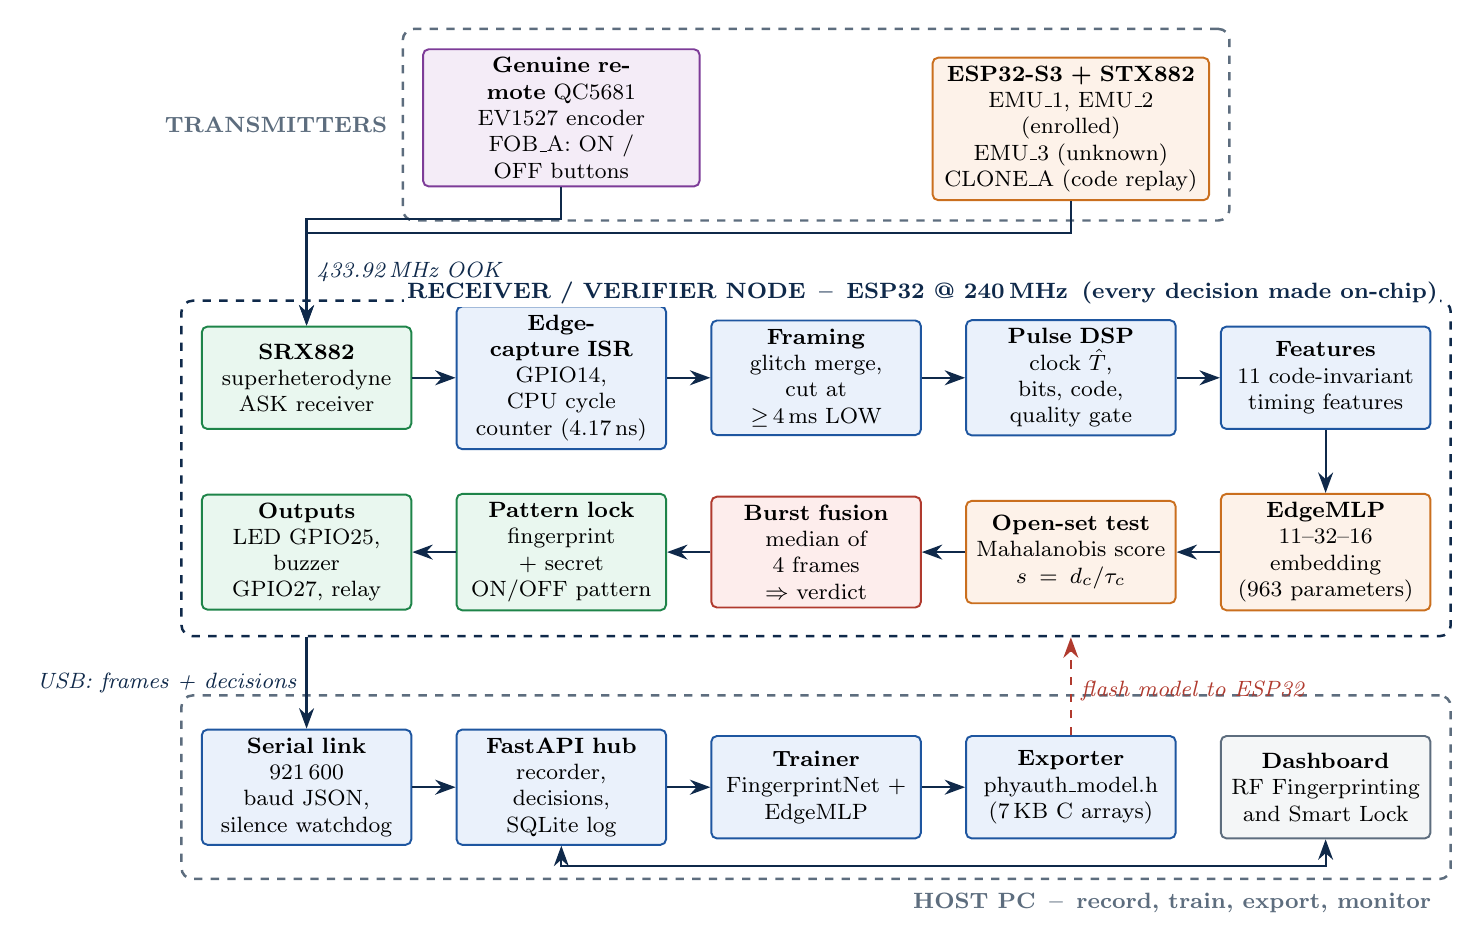
\begin{tikzpicture}[node distance=5mm and 5.5mm, every node/.style={font=\footnotesize}]
\tikzset{b/.style={blk=24.5mm, minimum height=13mm}}
% ---------------- receiver rows
\node[b, draw=grn, fill=lgrn] (rx) {\textbf{SRX882}\\superheterodyne\\ASK receiver};
\node[b, right=of rx] (isr) {\textbf{Edge-capture ISR}\\GPIO14, CPU cycle\\counter (4.17\,ns)};
\node[b, right=of isr] (frm) {\textbf{Framing}\\glitch merge,\\cut at $\geq$\,4\,ms LOW};
\node[b, right=of frm] (dsp) {\textbf{Pulse DSP}\\clock $\hat T$, bits, code,\\quality gate};
\node[b, right=of dsp] (feat) {\textbf{Features}\\11 code-invariant\\timing features};
\node[b, below=8mm of feat, draw=org, fill=lorg] (mlp) {\textbf{EdgeMLP}\\11--32--16 embedding\\(963 parameters)};
\node[b, left=of mlp, draw=org, fill=lorg] (maha) {\textbf{Open-set test}\\Mahalanobis score\\$s = d_c/\tau_c$};
\node[b, left=of maha, draw=red, fill=lred] (fus) {\textbf{Burst fusion}\\median of 4 frames\\$\Rightarrow$ verdict};
\node[b, left=of fus, draw=grn, fill=lgrn] (lock) {\textbf{Pattern lock}\\fingerprint + secret\\ON/OFF pattern};
\node[b, left=of lock, draw=grn, fill=lgrn] (io) {\textbf{Outputs}\\LED GPIO25, buzzer\\GPIO27, relay};
\foreach \a/\b in {rx/isr,isr/frm,frm/dsp,dsp/feat,feat/mlp,mlp/maha,maha/fus,fus/lock,lock/io} \draw[flow] (\a) -- (\b);
\begin{scope}[on background layer]
\node[frame=navy, fit=(rx)(feat)(io)(mlp), inner ysep=9pt] (rxf) {};
\end{scope}
\node[ttl=navy, anchor=south east, font=\footnotesize\bfseries, fill=white, inner sep=1pt] at ($(rxf.north east)+(-4pt,-3pt)$) {RECEIVER / VERIFIER NODE \,--\, ESP32 @ 240\,MHz \,(every decision made on-chip)};
% ---------------- transmitters (top)
\node[b, draw=pur, fill=lpur, above=15mm of isr, text width=33mm] (fob) {\textbf{Genuine remote} QC5681\\EV1527 encoder\\FOB\_A: ON / OFF buttons};
\node[b, draw=org, fill=lorg, above=15mm of dsp, text width=33mm] (emu) {\textbf{ESP32-S3 + STX882}\\EMU\_1, EMU\_2 (enrolled)\\EMU\_3 (unknown)\\CLONE\_A (code replay)};
\begin{scope}[on background layer]
\node[frame=gry, fit=(fob)(emu)] (txf) {};
\end{scope}
\node[ttl=gry, anchor=east, font=\footnotesize\bfseries] at (txf.west) {TRANSMITTERS\,};
\draw[flow] (fob.south) -- ++(0,-4mm) -| node[lbl, pos=0.75, right] {433.92\,MHz OOK} (rx.north);
\draw[flow] (emu.south) -- ++(0,-4mm) -| (rx.north);
% ---------------- host (bottom)
\node[b, below=15mm of io] (ser) {\textbf{Serial link}\\921\,600 baud JSON,\\silence watchdog};
\node[b, right=of ser] (hub) {\textbf{FastAPI hub}\\recorder, decisions,\\SQLite log};
\node[b, right=of hub] (trn) {\textbf{Trainer}\\FingerprintNet +\\EdgeMLP};
\node[b, right=of trn] (exp) {\textbf{Exporter}\\phyauth\_model.h\\(7\,KB C arrays)};
\node[b, right=of exp, draw=gry, fill=lgry] (ui) {\textbf{Dashboard}\\RF Fingerprinting\\and Smart Lock};
\foreach \a/\b in {ser/hub,hub/trn,trn/exp} \draw[flow] (\a) -- (\b);
\draw[flow, <->] (hub.south) -- ++(0,-2.6mm) -| (ui.south);
\begin{scope}[on background layer]
\node[frame=gry, fit=(ser)(ui), inner ysep=12pt] (hf) {};
\end{scope}
\node[ttl=gry, anchor=north east, font=\footnotesize\bfseries] at ($(hf.south east)+(-4pt,-1pt)$) {HOST PC \,--\, record, train, export, monitor};
\draw[flow] (rxf.south -| ser) -- node[lbl, left] {USB: frames + decisions} (ser.north);
\draw[flow, dashed, draw=red] (exp.north) -- node[lbl, right, text=red, pos=0.45] {flash model to ESP32} (rxf.south -| exp);
\end{tikzpicture}
\end{document}
